\documentclass[11pt]{article}
\usepackage[margin=1in]{geometry}
\usepackage[T1]{fontenc}
\usepackage{lmodern}
\usepackage{microtype}
\usepackage{amsmath,amssymb}
\usepackage{booktabs}
\usepackage{graphicx}
\usepackage{xcolor}
\usepackage[numbers,sort&compress]{natbib}
\usepackage[colorlinks=true,linkcolor=blue!50!black,citecolor=blue!50!black,urlcolor=blue!50!black]{hyperref}

% Placeholders for results still being measured. The build lists every remaining one.
\newcommand{\TODO}[1]{\textcolor{red}{[TODO: #1]}}
\newcommand{\pending}{\textcolor{red}{[pending]}}

\title{Switching Models Mid-Task Without Re-Reading:\\
Translating KV Caches Between Local Coding-Agent Models Through a Shared Latent}
\author{Ulises Rayon}
\date{}

\begin{document}
\maketitle

\begin{abstract}
A coding agent on one consumer machine often wants more than one model: a fast one to explore a
repository and a stronger one, such as Gemma~4~31B, to write the fix. Switching local models today
means the new model re-reads the whole session, tens of seconds of prefill on an integrated GPU. We
translate the session's attention cache instead. Closed-form linear adapters map each model's per-token
keys and values into a shared latent fitted by multi-view CCA (the \emph{hub}) and decode them into the
next model's cache, so $N$ models need $2N$ adapters and a new model joins by fitting only its own. One
hub spans 15 open models from seven cache families and 12 vocabularies, and a live switch between
llama.cpp servers is 1.4--6.8$\times$ faster than native prefill. On the competition's coding-agent
sessions, translation removes 16--38\% of the loss an information-free cache leaves, half of the rest
sits in template markup the hub does not cover, and fitting the hub on agent sessions raises the share into
Gemma from 19\% to 27\%. In 72 live hand-offs Gemma's
next tool call matched its native choice in 15 of 18 sessions, but an information-free cache did nearly
as well: on this sample the native tail, not the translation, carries the next step. Code and the hub
bundle are released.
\end{abstract}

% ---------------------------------------------------------------------------------------------
\section{Introduction}

Local coding agents are constrained less by any single model than by the context they carry. On the
Gemma~4 Developer Agent tasks a resolved Gemma~4~31B session holds a median of 14.7K tokens (Qwen3.8's:
15.8K, 90th percentile 20.3K) of tool calls, file excerpts, test output and reasoning. On consumer
hardware the prefill of that context, not generation, dominates the cost of changing models: re-reading
12K tokens takes about 50\,s for a 27B model on our integrated GPU (Section~\ref{sec:live}).

Yet a local agent wants to change models mid-task: small models explore quickly but write weak patches,
and Gemma~4~31B is the reverse. Cloud systems route per request because prefill is cheap for
them~\citep{chen2023frugalgpt,ong2024routellm}; prefix
caching~\citep{kwon2023vllm,zheng2024sglang,gim2024promptcache} helps only when the \emph{same} model sees
the prefix again. We ask whether the cache itself can be carried across models that differ in tokenizer,
depth, head layout, positional scheme and cache family. Our contributions:
\begin{enumerate}
\item A \emph{hub} for KV caches: per-token keys and values of $N$ models mapped into one
  shared latent by generalized CCA, with closed-form ridge encoders and decoders
  (Section~\ref{sec:hub}). Adding a model needs only its own captures; we document the
  calibration bias of the naive onboarding encoder and a per-dimension correction for it.
\item A switch protocol for running llama.cpp servers that keeps every token id exact and
  translates only old cache values, with byte alignment across tokenizers, a native tail, and a
  per-model mean recurrent state for hybrids (Section~\ref{sec:switch}).
\item An evaluation on 15 models and on the competition's coding-agent sessions, with bootstrap
  intervals, exact sign-flip tests and negative results (Sections~\ref{sec:setup}--\ref{sec:agents}): where the
  loss of a switch lives, agent-fitted hubs, and the next tool call after a live hand-off.
\item An open implementation (kvpark) that integrates with two agent front ends (Hermes and
  OpenCode) and runs entirely offline.
\end{enumerate}

% ---------------------------------------------------------------------------------------------
\section{Related work}

\paragraph{Reusing KV caches.} PagedAttention~\citep{kwon2023vllm}, RadixAttention~\citep{zheng2024sglang}
and Prompt Cache~\citep{gim2024promptcache} reuse a model's own cache for repeated prefixes;
CacheBlend~\citep{yao2025cacheblend} reuses caches of non-prefix chunks of the same model with
selective recomputation. DroidSpeak~\citep{liu2024droidspeak} shares caches between fine-tunes of
one base model.

\paragraph{Moving caches between different models.} Cache-to-Cache~\citep{fu2025c2c} fuses one
model's cache into another's with a trained neural projector for a fixed pair, and
KVComm~\citep{shi2026kvcomm} and activation communication~\citep{ramesh2025activations} let models
exchange selected internal states. Closest to us, \citet{dery2026kvalign} train adapters that map
the caches of several Gemma-2 models into one shared space, and CacheBridge~\citep{qu2026cachebridge}
fits closed-form affine maps from source to target heads for pairs within a model family. We
differ in three ways: our 15 models span seven cache families and 12 vocabularies, aligned by bytes; one
generalized-CCA latent serves every direction and onboards a model by fitting only its own adapters; and
translated caches are restored into unmodified llama.cpp servers during live coding-agent sessions.

\paragraph{Shared representations across models.} Representations of different networks are
related by largely linear maps~\citep{lenc2015equivariance,bansal2021stitching,kornblith2019cka,raghu2017svcca},
and larger models converge further~\citep{huh2024platonic}. Relative
representations~\citep{moschella2023relative} build a shared space from anchors. We use
multi-view CCA~\citep{kettenring1971gcca} on token-aligned caches, which yields one latent for
many models at once.

\paragraph{Coding agents.} SWE-bench~\citep{jimenez2024swebench}, SWE-agent~\citep{yang2024sweagent}
and OpenHands~\citep{wang2025openhands} established repository-level agent evaluation;
SWE-smith~\citep{yang2025swesmith} synthesizes training tasks. Model cascades and
routing~\citep{chen2023frugalgpt,ong2024routellm} choose a model per request. We make the
choice cheap to change \emph{within} a session on local hardware.

% ---------------------------------------------------------------------------------------------
\section{Method}\label{sec:method}

\subsection{What a switch must produce}
When a conversation moves from model $A$ to model $B$, $B$'s server renders it with $B$'s own template and
tokenizer. We write $B$'s cache for its first $T_0 = P - W$ tokens of a $P$-token prompt and let $B$ prefill
the native tail of $W = 2{,}048$ tokens, never past the newest message. llama.cpp reuses only cells whose
token ids match the request, so $B$ always conditions on the right tokens; translation changes only the
values of old cache rows.

\subsection{The hub}\label{sec:hub}
\paragraph{Alignment.} A \emph{hub span} is a token that ends at the same byte of the same message in every
model's rendering; renderings are aligned on bytes, never on token ids (the 15 models use 12 vocabularies).

\paragraph{Views.} For model $m$, the pre-RoPE keys (and separately the values) of all its attention layers
at a span are reduced by per-layer PCA to at most 512 components, concatenated and reduced to a whitened view
$x_m \in \mathbb{R}^{d}$, $d = 4{,}096$. Keys are de-rotated with the source's own positional scheme (full or
partial NeoX, M-RoPE, interleaved on MLA, NoPE), so the hub holds position-free keys and the target
re-rotates. Sliding-window sources encode from their global layers alone; an MLA model's key view is its
latent row $[c_{kv} \mid k_{pe}]$.

\paragraph{Fitting.} The latent $z$ is the MAXVAR generalized-CCA consensus of the base models'
views~\citep{kettenring1971gcca}, a generalized eigenproblem with each view block whitened by its training
covariance. Encoders $E_m$ are ridge regressions from each view to $z$; the decoder $D_n$ regresses every
cache layer of model $n$ on the pooled encoder estimates of all \emph{other} models, so any source works at
run time. Nothing is trained by gradient descent. A switch computes $D_B(E_A(x_A))$ per span and re-rotates
$B$'s keys at $B$'s positions.

\paragraph{Onboarding.} A new model is added without changing existing adapters: its decoder regresses its
cache on the base models' pooled latent estimates, and its encoder regresses its view on their mean
estimate. That mean is the consensus shrunk per dimension, so a plain ridge encoder yields latents with about
half the spread of a jointly fitted model's: held-out $R^2$ barely notices, but decoded keys lose variance and
attention flattens. Our \texttt{reverse} encoder rescales each dimension by
$\mathrm{var}(z_j)/\mathrm{cov}(z_j,\hat z_j)$, capped at $4\times$, which makes the encoding unbiased given
the target. Into Qwen3.8 it raised the share of the floor's loss removed from 3/4/11\% to 17/24/41\% for
DeepSeek-V2-Lite, LFM2 and Qwen3.6.

\subsection{Cells the hub does not cover}\label{sec:switch}
Template and special tokens, and text tokenized so that no span is shared, have no hub estimate and are
filled with the decoder's training mean. Per target, the system message can be prefilled natively, since
the first tokens act as an attention sink. Linear-attention and Mamba hybrids also carry a fixed-size
recurrent state that cannot be translated per token; it starts from the model's mean native state and the
native tail carries it forward. Switches the translator cannot handle are skipped with a reason code and the
target prefills natively; a model that translates out worse than no translation is registered as a target
only.

% ---------------------------------------------------------------------------------------------
\section{Experimental setup}\label{sec:setup}

\paragraph{Machine.} One AMD Ryzen AI Max+ 395 with a Radeon 8060S integrated GPU and 128\,GB of
unified memory, llama.cpp a7b94df2c on Vulkan (and the production build 85d5703a3 for live
switches into Qwen3.8). CPU and GPU share one cooler, so a
thermal guard pauses work above 90\,\textdegree C; timings exclude its pauses.

\paragraph{Models.} The hub's base views are Qwen3.8-27B (gated-DeltaNet hybrid), Muse-Glimmer-30B
(sliding window), Qwen3-4B (dense GQA) and Ornith-1.5-9B (hybrid). Twelve models were onboarded
(Table~\ref{tab:chat}), among them Gemma~4 26B-A4B and Gemma~4 31B, the competition's model; eleven are
in the final hub (Jamba is excluded). Weights are Q8\_0 except Gemma~4 (QAT UD-Q4\_K\_XL), GLM-4.7-Flash
(Q5\_K\_M) and Kimi-Linear (Q4\_K\_M).

\paragraph{Metric.} For each held-out conversation the target restores the translated cache for
$[0,T_0)$, prefills the native tail, and is scored teacher-forced on the first 256 tokens of the
final message against its own full prefill. The \emph{floor} fills every translated cell with the
decoder mean (no information from the source, same native tail). We report the share of the
floor's KL divergence the translation removes, $1 - \mathrm{KL}_{\text{hub}}/\mathrm{KL}_{\text{floor}}$,
token-weighted, with 95\% document-bootstrap intervals and exact paired sign-flip tests. The target's own native cache scores exactly zero.

\paragraph{Corpora.} \emph{Chat}: held-out long multi-turn conversations (4.5--16K tokens) from
SmolTalk2. \emph{Coding agent}: resolved trajectories on the competition's development tasks
(21 resolved sessions per model, one per task, from 22 tasks on FastAPI, Requests and HTTPX; 18 of each are
long enough to evaluate) and, for fitting only, SWE-smith sessions~\citep{yang2025swesmith} on repositories disjoint
from those. Each trajectory is cut at the first
assistant turn past half its length; the scored message is that turn's reasoning and tool call.
Renderings follow llama-server's, as a live switch holds them.

% ---------------------------------------------------------------------------------------------
\section{Results on chat}\label{sec:chat}

\paragraph{One latent for many models.} With four base models and three tokenizers, translated
keys reach held-out $R^2$ 0.67--0.77 and values 0.49--0.67 in all twelve directions, 97\%/93\% of a
dedicated pairwise map for the same pair. The top canonical eigenvalues are 3.99 and 3.98 of a
possible 4: the leading directions are shared almost perfectly. Figure~\ref{fig:r2} extends this to
all 15 models: between onboarded models, which never saw each other's captures, keys reach $R^2$
0.35--0.75.

\begin{figure}[t]
\centering
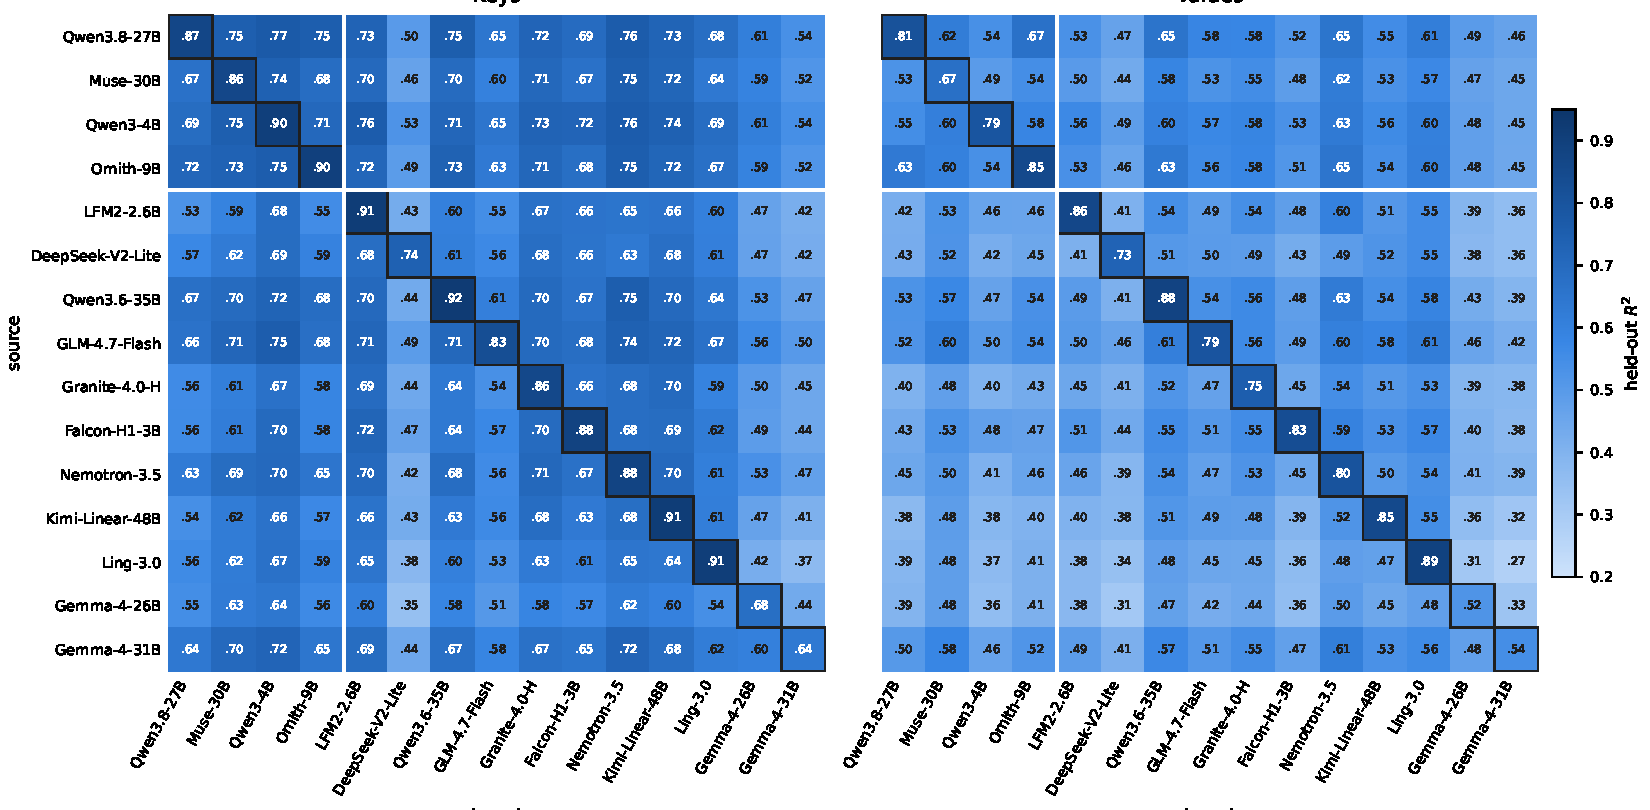
\includegraphics[width=\linewidth]{figures/r2.pdf}
\caption{Held-out $R^2$ of translated keys and values for every ordered pair of the 15 hub models
(8,699 test spans shared by all; the white rule separates the four jointly fitted base models from the
onboarded ones; diagonal: a model's own cache through the hub).}
\label{fig:r2}
\end{figure}

% Source: evidence/universal-kv/review-20261009/tables.md (hub6-20261009; templates' own rendering).
% "Into": Qwen3.8 -> model, the six held-out chats every run shares. "Out of": model -> Qwen3.8, eight chats.
\begin{table}[t]
\centering
\small
\caption{Long held-out chats (4.5--16K tokens): share of the information-free floor's KL removed by a
switch, with 95\% document-bootstrap intervals and exact paired sign-flip $p$. Base models (fitted
jointly) above the rule, onboarded models below. $^\dagger$: \texttt{ridge} encoder (the default
\texttt{reverse} encoder did no good or harm). --: not in the hub.}
\label{tab:chat}
\resizebox{\linewidth}{!}{%
\begin{tabular}{llll}
\toprule
Model & Cache family & Into the model (from Qwen3.8) & Out of the model (into Qwen3.8) \\
\midrule
Qwen3-4B & dense GQA & -- & 30\% (reference) \\
\midrule
GLM-4.7-Flash & MLA & 83\% [80, 84], $p$ .031 & 38\% [23, 46], $p$ .008 \\
Ling-3.0-tiny & MLA + linear attn. & 71\% [64, 75], $p$ .031 & 42\% [29, 48], $p$ .016 \\
LFM2-2.6B & conv. hybrid & 51\% [45, 65], $p$ .031 & 24\% [13, 32], $p$ .023 \\
Qwen3.6-35B-A3B & DeltaNet hybrid, MoE & 50\% [37, 55], $p$ .031 & 41\% [20, 54], $p$ .016 \\
Gemma-4-26B-A4B & sliding + global GQA & 45\% [31, 48], $p$ .031 & 37\% [17, 50], $p$ .016 \\
Gemma-4-31B & sliding + global GQA & 35\% [27, 51], $p$ .031 & 33\% [16, 44], $p$ .008 \\
DeepSeek-V2-Lite & MLA & 31\% [28, 34], $p$ .031 & 17\% [9, 23], $p$ .031 \\
Kimi-Linear-48B-A3B & MLA + linear attn. & 21\% [19, 24], $p$ .031 & 32\% [15, 45], $p$ .023 \\
Nemotron-3.5-30B-A3B & Mamba hybrid & 16\% [12, 30], $p$ .031 & 5\%$^\dagger$ [3, 8]; $-44\%$ as served \\
Falcon-H1-3B & Mamba hybrid & 9.5\% [8, 10], $p$ .094 & 25\% [13, 33], $p$ .055 \\
Granite-4.0-H-Tiny & Mamba hybrid & 6.3\% [$-2$, 8], $p$ .25 & 1.3\%$^\dagger$ [0.6, 2.3] \\
Jamba-Reasoning-3B & Mamba hybrid & 6.8\% [$-1$, 18], $p$ .22 & $-1031\%$ (--) \\
\bottomrule
\end{tabular}}
\end{table}


\paragraph{End to end.} Table~\ref{tab:chat}. Translations into the new models
remove 16--83\% of the floor's KL for nine of twelve; out of them into Qwen3.8, 25--42\% where the
onboarding is well conditioned (Qwen3-4B, fitted jointly: 30\%).

\paragraph{Negative results.} (i) A seven-model joint refit did worse than onboarding out of all
four sources tested. (ii) For Mamba hybrids with few attention layers the onboarded encoder is
ill-conditioned: Granite gains nothing, Jamba is destructive, and Nemotron remains harmful as a
source even with a plain ridge encoder ($-44\%$), so it is registered as a target only. (iii)
Held-out $R^2$ does not predict switch quality: Nemotron's ridge encoder has among the highest.

% ---------------------------------------------------------------------------------------------
% Source: paper/data/pilot.json (paper/scripts/agent_stats.py over evidence/universal-kv/swe-agent-pilot/ and
% campaign/gemma-4-31b/eval/*-server). Deployed setting: native prompt start (system message and tool schemas).
\begin{table}[t]
\centering
\small
\caption{The same model pair on chat and on coding-agent sessions (hub6, server rendering, 2,048-token
native tail, native prompt start). Agent: 18 of Gemma~4~31B's resolved sessions, cut half way and scored on the
next reasoning and tool call. Nats per token over 256 scored tokens; 95\% document-bootstrap intervals; $p$:
exact paired sign-flip test.}
\label{tab:agent}
\resizebox{\linewidth}{!}{%
\begin{tabular}{llcccc}
\toprule
Direction & Sessions & Floor KL & Translated KL & Translated $\Delta$NLL & Floor KL removed \\
\midrule
Qwen3.8 $\to$ Gemma~4~31B & chat (6) & 0.072 & 0.046 & $+0.022$ [$-0.001$, 0.044] & 36\% [23, 50], $p$ .031 \\
 & agent (18) & 0.365 & 0.308 & $+0.315$ [0.146, 0.526] & 16\% [5, 24], $p$ .012 \\
Gemma~4~31B $\to$ Qwen3.8 & chat (8) & 0.068 & 0.045 & $+0.033$ [0.010, 0.065] & 34\% [18, 43], $p$ .008 \\
 & agent (18) & 0.163 & 0.102 & $+0.094$ [0.031, 0.167] & 38\% [2, 49], $p$ .058 \\
\bottomrule
\end{tabular}}
\end{table}

% Source: paper/data/live.json (paper/scripts/live_stats.py over evidence/universal-kv/swe-agent-live/*).
\begin{table}[t]
\centering
\small
\caption{Live hand-offs of 18 agent sessions per direction (the target's own, 4.6--13.6K tokens): the
target's next call at temperature 0 after a switch, against its call after a native prefill and the call the
session made. Floor: a hub copy with the target's decoders zeroed. Speed-up: native prefill over switch plus
tail, guard pauses removed, median [range].}
\label{tab:live}
\resizebox{\linewidth}{!}{%
\begin{tabular}{llccccc}
\toprule
 & & \multicolumn{3}{c}{vs.\ native next call} & vs.\ session & \\
\cmidrule(lr){3-5}
Direction & Cache & Tool & Target & Identical & Tool / identical & Speed-up \\
\midrule
Qwen3.8 $\to$ Gemma~4~31B & hub & 15 & 8 & 5 & 11 / 6 & 2.2$\times$ [2.0, 3.0] \\
 & floor & 14 & 10 & 4 & 11 / 4 & 2.2$\times$ [2.0, 2.8] \\
 & native & -- & -- & -- & 13 / 10 & 1 \\
Gemma~4~31B $\to$ Qwen3.8 & hub & 12 & 6 & 1 & 10 / 0 & 2.9$\times$ [1.4, 3.9] \\
 & floor & 11 & 5 & 1 & 11 / 1 & 2.9$\times$ [1.4, 4.0] \\
 & native & -- & -- & -- & 11 / 1 & 1 \\
\bottomrule
\end{tabular}}
\end{table}

% Source: paper/data/decompose.json (paper/scripts/decompose_stats.py over
% evidence/universal-kv/swe-agent-decompose/qwen38-to-gemma-4-31b).
\begin{table}[t]
\centering
\small
\caption{Where the loss of a switch into Gemma~4~31B lives (Qwen3.8 $\to$ Gemma, 12 agent sessions, KL
0.335, floor 0.502). An oracle gives Gemma its native values for one class of translated tokens; share of the
remaining KL removed, 95\% document-bootstrap intervals. Classes overlap.}
\label{tab:decompose}
\begin{tabular}{lcc}
\toprule
Class made native & Tokens & KL removed \\
\midrule
Fill (no hub estimate: markup, special tokens) & 24\% & 49\% [36, 62] \\
Reasoning & 6\% & 35\% [8, 55] \\
Tool output & 15\% & 30\% [4, 50] \\
Tool-call arguments & 3\% & 10\% [1, 17] \\
\midrule
The 2,048 tokens before the native tail & 49\% & 50\% [33, 68] \\
\bottomrule
\end{tabular}
\end{table}


\section{Coding-agent sessions}\label{sec:agents}

\paragraph{The chat-fitted hub on agent sessions.} Table~\ref{tab:agent} evaluates the same hub on Gemma~4~31B's
resolved sessions on the competition's development tasks. Translation still helps in both directions, but the floor
is 2.4--5 times higher: on chat the last 2,048 tokens carry most of what the next reply needs, while an agent's next
action depends on file contents, test output and its own edits far back in the context. Into Gemma the share
recovered also drops (16\% against 36\% on chat), so a switch costs $+0.32$ nats per token against $+0.02$ on chat;
out of Gemma into Qwen3.8 the share holds (38\%, $+0.09$).

\paragraph{Where the loss lives.} An oracle gives Gemma its own native values for one class of translated tokens
at a time (Table~\ref{tab:decompose}). Half of the loss sits in
the fill cells, the template markup and special tokens the hub has no estimate for and fills with a mean: they are a
quarter of the tokens. Per token, reasoning and tool-call arguments are the densest (6\% of the tokens carry
35\%, and 3\% carry 10\%); tool output, the bulk of an agent's context, carries about twice its share. A native
tail twice as long would remove half the loss, at the price of prefilling 2,048 more tokens. The next
improvement is the fill, not the hub: the per-token-id table we use for other targets fails on Gemma (KL above 4).

\paragraph{Fitting the hub on agent sessions.} We fit two two-model hubs (Qwen3.8 and Gemma~4~31B) with hub6's
settings: one on the chat captures alone, one on the same plus 11 SWE-smith sessions on repositories disjoint from the
evaluation tasks, which doubles the training spans.
Into Gemma, the agent-fitted hub removes 27\% [14, 39] of the floor's KL on the 18 agent sessions in the deployed
setting, against 19\% [8, 27] for the chat-fitted one: 11\% less KL [3, 25], better on 13 of 18 sessions ($p$ .013).
It costs on chat: on the six held-out chats the share falls from 35\% to 28\% (0 of 6 better, $p$ .031). Domain
matters, so a deployment would fit its hub on the sessions it expects. The reverse direction is not measured.

\paragraph{Does the next action survive?} Teacher-forced loss does not show whether the agent still acts
right. We hand live sessions between two running llama.cpp servers (Qwen3.8 and Gemma~4~31B, the bridge's GPU
engine) and let the target produce the next turn at temperature 0, after a native prefill and after a switch, with
the session's tools in the request (Table~\ref{tab:live}). All 72 switches reused exactly the translated prefix.
After a switch from Qwen3.8, Gemma chose the same tool as after a native prefill in 15 of 18 sessions, the same file
or command in 8 and an identical call in 5. Of the 13 that differ, 6 repeat the read or search with another
range, 5 take another plausible step, and 2 look like lost context.

The floor shows how much of this the translation earns: not measurably. With the target's decoders zeroed, Gemma
still chose the same tool in 14 sessions and the same target in 10; into Qwen3.8 hub and floor agree with native on
12 and 11 tools. With 18 sessions and a 2,048-token tail, the next action is carried by the tail and the prompt start.
So a switch is safe for the next step even when translation is weak, and the 16\% of the loss the hub removes into
Gemma is real but too small to move a discrete decision on this sample.

\paragraph{Speed.} Translating 4.3--8.2K cached tokens took 1.1--1.8\,s on the GPU, once Gemma~4~31B's decoder was
split under the Vulkan 1\,GiB buffer limit (otherwise it fell back to the CPU, 47\,s). Without guard
pauses, a switch plus the native tail into Gemma took a median 9.0\,s against 20.7\,s of native prefill
(2.0--3.0$\times$); into Qwen3.8, 6.7\,s against 19.2\,s (1.4--3.9$\times$). The ratio grows with length since the tail is fixed. Gemma's prompt start (system prompt and tool schemas) is prefilled natively once, 13.7\,s,
and cached for later sessions with the same tools.

% ---------------------------------------------------------------------------------------------
\section{Live switches on chat}\label{sec:live}
In ten live switches between running servers (8--15K tokens), every switch reused exactly the translated prefix.
Into Qwen3.8 a switch took 9.7--12.5\,s against 48--52\,s of native prefill (3.3--6.8$\times$); into Gemma~4~26B
2.0--3.1$\times$. Translation takes 0.45--1.8\,s; the rest is the native tail.

% ---------------------------------------------------------------------------------------------
\section{Limitations}
Scores are teacher-forced on the first 256 tokens of one message per conversation. The chat
evaluation reuses the conversations on which onboarding methods were chosen. Some intervals rest
on few documents and one conversation dominates three targets' pooled scores. All measurements are
from one machine. The agent evaluation covers one model pair, 18 sessions per direction on three
repositories, and the next call only, not task completion after a hand-off; with that sample the live comparison
cannot separate the hub from the floor. The agent-fitted hub is measured into Gemma only, and its gain is not
separated from that of doubling the training data.

\section{Conclusion}
One linear latent carries attention caches between 15 local models, and a live switch makes a model change
mid-session cost seconds instead of a re-read. On coding-agent sessions the translation is weaker than on chat, and
on our sample the next tool call is held up by the native tail rather than by the translation. The decomposition says
where to work next: the template markup the hub does not cover, and the agent's reasoning; fitting on agent
sessions already helps, at a small cost on chat.

\paragraph{Availability.} Code, evaluation scripts and the paper's tables are at
\url{https://github.com/uncrayon/kvpark} (MIT); the 15-model hub bundle (f16, 17.7\,GB) is at \url{https://huggingface.co/uncrayon/kvpark-hub6} and attached
to the repository's release.

\bibliographystyle{plainnat}
\bibliography{refs}
\end{document}
